\documentclass[ngerman,a4paper]{report}
\usepackage[ngerman]{babel}
\usepackage[T1]{fontenc}
\usepackage[utf8]{inputenc}
\usepackage{MyriadPro}
\usepackage[scaled]{beramono}
\newcommand\Small{\fontsize{10.5}{10.5}\selectfont}
\newcommand*\LSTfont{\Small\ttfamily\SetTracking{encoding=*}{-20}\lsstyle}
\usepackage{microtype}
\usepackage{geometry}
\geometry{verbose,tmargin=3cm,bmargin=3cm,lmargin=3cm,rmargin=3cm}
\usepackage{listings}
\usepackage{stmaryrd}
\usepackage{paralist}
\usepackage{array}
\usepackage{color}
\usepackage{graphicx}
\usepackage{caption}
\usepackage{url}
\usepackage{amsmath}
\usepackage{accents}
\usepackage{tikz}
\usetikzlibrary{plotmarks}

% Code Listing Style
\definecolor{darkblue}{rgb}{0,0,.6}
\definecolor{darkgreen}{rgb}{0,0.5,0}
\definecolor{darkred}{rgb}{0.5,0,0}
\lstset{%
	language=[x86masm]Assembler, 
	basicstyle=\LSTfont,
	commentstyle=\color{darkgreen}, 
	keywordstyle=\color{darkblue}\bfseries, 
	breaklines=true,
	tabsize=2,
	xleftmargin=\fboxsep,
	xrightmargin=-\fboxsep,
	numbers=left,
	numberstyle=\tiny\color{gray},
	stepnumber=1,
	numbersep=5pt,
	frame=bt,
	stringstyle=\color{darkred},
	showstringspaces=false,
	rulecolor= \color{gray},
	emph=[1]%
	{%  
	    then, not, for, return%
	},
	emphstyle=[1]{\color{darkblue}\bfseries},
	emph=[2]%
	{%  Datatypes
	    %
	},
	emphstyle=[2]{\color{darkblue}\bfseries},
	emph=[3]%
	{%  
	    %
	},
	emphstyle=[3]{\color{darkred}\bfseries},
	literate=%
	{Ö}{{\"O}}1
	{Ä}{{\"A}}1
	{Ü}{{\"U}}1
	{ß}{{\ss}}2
	{ü}{{\"u}}1
	{ä}{{\"a}}1
	{ö}{{\"o}}1
}
\providecommand{\tabularnewline}{\\}

\usepackage{fancyhdr}
\pagestyle{fancy}
\usepackage{lastpage}
\makeatletter

\lhead{\textbf{\@title} \\ \@author}
\chead{}
\rhead{\@date \\ \thepage \ von \pageref{LastPage} }
\cfoot{}

\renewcommand{\maketitle}{}
\newcommand{\utilde}[1]{\underaccent{\tilde}{#1}}
\renewcommand{\familydefault}{\sfdefault}
 
\author{Tobias Höppner}
\title{HA - Übung 05.}
\date{Wintersemester 2014/2015}

\begin{document} 
\maketitle 

\subsubsection*{29. Programmieraufgabe: Multiplikation langer Zahlen nach Karatsuba, 20 Punkte}
Anmerkung zum Programmstart:
\begin{lstlisting}
java -jar Uebung.jar <ZAHL1> <ZAHL2>
\end{lstlisting}
Multipliziert \lstinline!ZAHL1! mit \lstinline!ZAHL2!.\\

Quellenangabe zur verwendeten Karatsuba Implementierung: \url{http://introcs.cs.princeton.edu/java/78crypto/Karatsuba.java.html}
Autoren:  Robert Sedgewick, Kevin Wayne.\\

Der Code wurde noch etwas angepasst. Da die Additionsoperation nicht von \lstinline!java.math.BigInteger! verwendet werden durfte. Ich habe mich entschieden diesen Code zu verwenden, weil er in der Länge und Struktur sehr kurz war und damit wenig Fehleranfällig. Im Quelltext finden sich noch zwei weitere Funktionen(\lstinline!nextBigInt(int n)! und \lstinline!test(int n)!) die ich zu Testzwecken selbst geschrieben habe. Die verwendete Additionsmethode stellte sich als wenig effizient heraus. 
\subsubsection*{Messdaten}
%Daten:
%\begin{tabular}{|c|c|}
%\hline
%N & ms\\
%\hline
%1000 & 20\\
%\hline
%2000 & 27\\
%\hline
%3000 & 25\\
%\hline
%4000 & 41\\
%\hline
%5000 & 44\\
%\hline
%6000 & 67\\
%\hline
%7000 & 121\\
%\hline
%8000 & 124\\
%\hline
%9000 & 125\\
%\hline
%10000 & 132\\
%\hline
%11000 & 145\\
%\hline
%12000 & 203\\
%\hline
%13000 & 302\\
%\hline
%14000 & 357\\
%\hline
%15000 & 370\\
%\hline
%16000 & 369\\
%\hline
%17000 & 371\\
%\hline
%18000 & 372\\
%\hline
%19000 & 376\\
%\hline
%20000 & 396\\
%\hline
%21000 & 403\\
%\hline
%22000 & 433\\
%\hline
%23000 & 509\\
%\hline
%24000 & 610\\
%\hline
%25000 & 747\\
%\hline
%26000 & 909\\
%\hline
%27000 & 1034\\
%\hline
%28000 & 1104\\
%\hline
%29000 & 1127\\
%\hline
%30000 & 1175\\
%\hline
%31000 & 1143\\
%\hline
%32000 & 1216\\
%\hline
%33000 & 1152\\
%\hline
%34000 & 1183\\
%\hline
%35000 & 1187\\
%\hline
%36000 & 1190\\
%\hline
%37000 & 1205\\
%\hline
%38000 & 1246\\
%\hline
%39000 & 1192\\
%\hline
%40000 & 1217\\
%\hline
%41000 & 1223\\
%\hline
%42000 & 1237\\
%\hline
%43000 & 1273\\
%\hline
%44000 & 1305\\
%\hline
%45000 & 1413\\
%\hline
%46000 & 1528\\
%\hline
%47000 & 1672\\
%\hline
%48000 & 1833\\
%\hline
%49000 & 2027\\
%\hline
%50000 & 2291\\
%\hline
%51000 & 2527\\
%\hline
%52000 & 2778\\
%\hline
%53000 & 3000\\
%\hline
%54000 & 3150\\
%\hline
%55000 & 3182\\
%\hline
%56000 & 3238\\
%\hline
%57000 & 3291\\
%\hline
%58000 & 3308\\
%\hline
%59000 & 3331\\
%\hline
%60000 & 3354\\
%\hline
%61000 & 3356\\
%\hline
%62000 & 3358\\
%\hline
%63000 & 3374\\
%\hline
%64000 & 3361\\
%\hline
%65000 & 3360\\
%\hline
%66000 & 3369\\
%\hline
%67000 & 3364\\
%\hline
%68000 & 3359\\
%\hline
%69000 & 3389\\
%\hline
%70000 & 3366\\
%\hline
%71000 & 3353\\
%\hline
%72000 & 3371\\
%\hline
%73000 & 3382\\
%\hline
%74000 & 3389\\
%\hline
%75000 & 3396\\
%\hline
%76000 & 3414\\
%\hline
%77000 & 3446\\
%\hline
%78000 & 3493\\
%\hline
%79000 & 3558\\
%\hline
%80000 & 3609\\
%\hline
%81000 & 3580\\
%\hline
%82000 & 3600\\
%\hline
%83000 & 3593\\
%\hline
%84000 & 3636\\
%\hline
%85000 & 3675\\
%\hline
%86000 & 3746\\
%\hline
%87000 & 3801\\
%\hline
%88000 & 3915\\
%\hline
%89000 & 4070\\
%\hline
%90000 & 4221\\
%\hline
%91000 & 4404\\
%\hline
%92000 & 4580\\
%\hline
%93000 & 4819\\
%\hline
%94000 & 5033\\
%\hline
%95000 & 5256\\
%\hline
%96000 & 5533\\
%\hline
%97000 & 5776\\
%\hline
%98000 & 6037\\
%\hline
%99000 & 6406\\
%\hline
%100000 & 6831\\
%\hline
%\end{tabular}
%
%\begin{tabular}{|c|c|}
%\hline
%N & ms\\
%\hline
%1000 & 35\\
%\hline
%2000 & 54\\
%\hline
%3000 & 83\\
%\hline
%4000 & 148\\
%\hline
%5000 & 173\\
%\hline
%6000 & 250\\
%\hline
%7000 & 412\\
%\hline
%8000 & 443\\
%\hline
%9000 & 464\\
%\hline
%10000 & 515\\
%\hline
%11000 & 569\\
%\hline
%12000 & 744\\
%\hline
%13000 & 1052\\
%\hline
%14000 & 1232\\
%\hline
%15000 & 1297\\
%\hline
%16000 & 1343\\
%\hline
%17000 & 1360\\
%\hline
%18000 & 1396\\
%\hline
%19000 & 1452\\
%\hline
%20000 & 1556\\
%\hline
%21000 & 1604\\
%\hline
%22000 & 1715\\
%\hline
%23000 & 1970\\
%\hline
%24000 & 2257\\
%\hline
%25000 & 2700\\
%\hline
%26000 & 3195\\
%\hline
%27000 & 3589\\
%\hline
%28000 & 3759\\
%\hline
%29000 & 3861\\
%\hline
%30000 & 3994\\
%\hline
%31000 & 4025\\
%\hline
%32000 & 4095\\
%\hline
%33000 & 4155\\
%\hline
%34000 & 4178\\
%\hline
%35000 & 4230\\
%\hline
%36000 & 4206\\
%\hline
%37000 & 4261\\
%\hline
%38000 & 4371\\
%\hline
%39000 & 4523\\
%\hline
%40000 & 4689\\
%\hline
%41000 & 4776\\
%\hline
%42000 & 4856\\
%\hline
%43000 & 5014\\
%\hline
%44000 & 5211\\
%\hline
%45000 & 5556\\
%\hline
%46000 & 5918\\
%\hline
%47000 & 6273\\
%\hline
%48000 & 6752\\
%\hline
%49000 & 7384\\
%\hline
%50000 & 8133\\
%\hline
%51000 & 8923\\
%\hline
%52000 & 9737\\
%\hline
%53000 & 10240\\
%\hline
%54000 & 10696\\
%\hline
%55000 & 11062\\
%\hline
%56000 & 11289\\
%\hline
%57000 & 11510\\
%\hline
%58000 & 11675\\
%\hline
%59000 & 11921\\
%\hline
%60000 & 11978\\
%\hline
%61000 & 11898\\
%\hline
%62000 & 11986\\
%\hline
%63000 & 12030\\
%\hline
%64000 & 12139\\
%\hline
%65000 & 12338\\
%\hline
%66000 & 12301\\
%\hline
%67000 & 12423\\
%\hline
%68000 & 12372\\
%\hline
%69000 & 12548\\
%\hline
%70000 & 12556\\
%\hline
%71000 & 12654\\
%\hline
%72000 & 12692\\
%\hline
%73000 & 12788\\
%\hline
%74000 & 12859\\
%\hline
%75000 & 12970\\
%\hline
%76000 & 13182\\
%\hline
%77000 & 13370\\
%\hline
%78000 & 13633\\
%\hline
%79000 & 14024\\
%\hline
%80000 & 14812\\
%\hline
%85000 & 15452\\
%\hline
%90000 & 17154\\
%\hline
%95000 & 20241\\
%\hline
%100000 & 25033\\
%\hline
%\end{tabular}

\begin{figure}[h]
    \begin{center}
        %TODO
        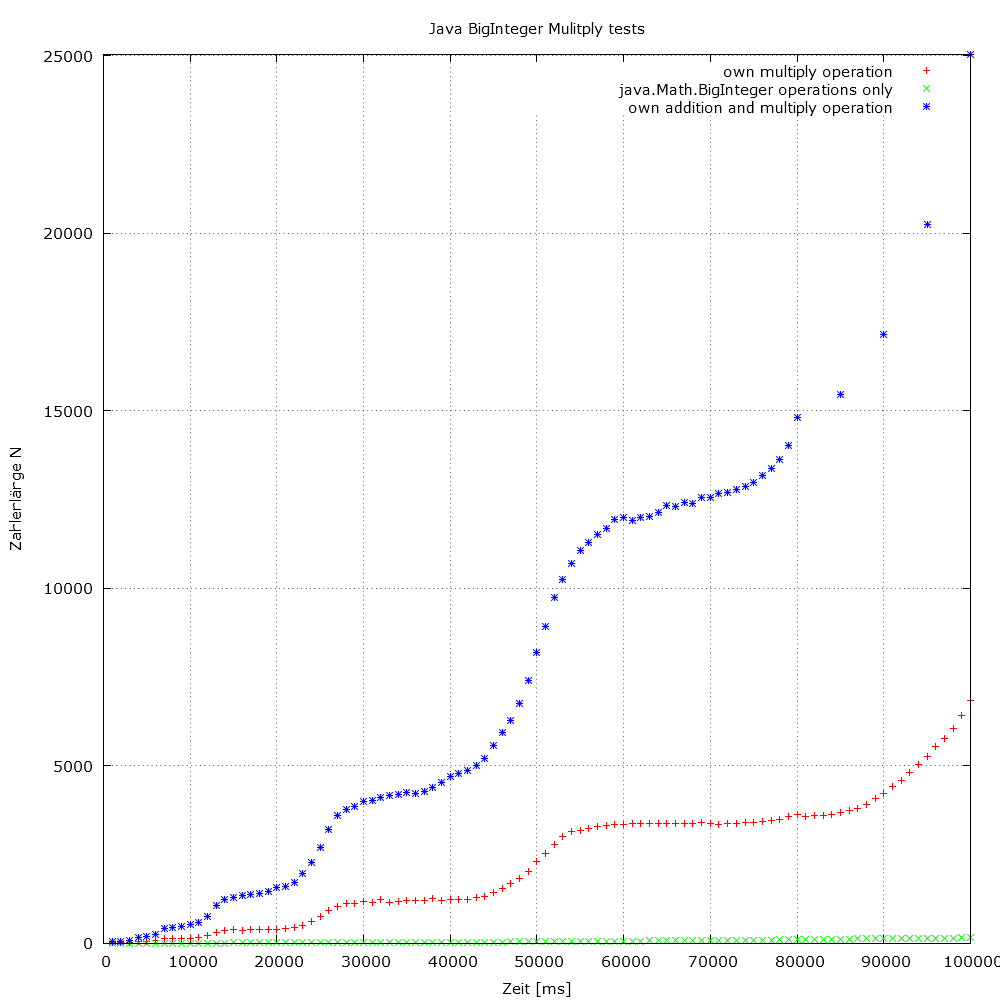
\includegraphics[width=360px]{testdaten.png}
    \end{center}
\end{figure}
Es wurden 3 Messreihen durchgeführt. Man erkennt deutlich, dass die Java internen Funktionen deutlich besser sind. \\
\newpage
\subsubsection*{Laufzeit}
Für die Laufzeit habe ich folgendes Datenpaar gewählt: $n = 100000 = 25033$ms.\\
Für $\alpha = 1$ ergibt sich:
\begin{align*}
25033 &= C * 100000^1\\
C &= 0.25033\\
\end{align*}

\end{document}
